\documentclass[10pt]{beamer}

\usetheme{Madrid}

% ------------------ Couleurs personnalisées ---------------------
\definecolor{P8blue}{RGB}{0,45,114}
\definecolor{P8light}{RGB}{230,235,245}
\definecolor{ProblemRed}{RGB}{180,15,25}

% Accentuation visuelle
\setbeamercolor{structure}{fg=P8blue}
\setbeamercolor{frametitle}{bg=P8blue!10, fg=P8blue}
\setbeamercolor{title}{fg=P8blue}
\setbeamercolor{titlepage}{fg=P8blue}

% Titres parfaitement lisibles
\setbeamercolor{.                         titlelike}{fg=P8blue}
\setbeamerfont{title}{series=\bfseries, size=\LARGE}

% Blocs
\setbeamercolor{block title}{bg=P8blue!20, fg=P8blue}
\setbeamercolor{block body}{bg=P8light!40}

\setbeamertemplate{navigation symbols}{}
\setbeamertemplate{footline}[frame number]
\setbeamercolor{title}{fg=white}
\setbeamercovered{transparent}


% Packages
\usepackage[T1]{fontenc}
\usepackage[utf8]{inputenc}
\usepackage[french]{babel}
\usepackage{graphicx}
\usepackage{array}
\usepackage{hyperref}

% ----------- MÉTADONNÉES -------------------
\title{\textbf{CarryBot}\\\large Robot compagnon d’assistance pour transport d’objets légers en intérieur}
\author{Lena BESSA — Zhaoyu WANG — Xinqi TANG — Lou LOPEZ}
\institute{Master 2 MIASHS — Technologie \& Handicap\\Université Paris 8}
\titlegraphic{
\includegraphics[height=2.5cm]{images/logo-p8.jpg} 
\hspace{2cm} 
\includegraphics[height=2.5cm]{images/logo-handi.png}}

\usepackage[numbers]{natbib}
\bibliographystyle{unsrt}
% -------------------------------------------------------------
\begin{document}
% -------------------------------------------------------------

% -------------------------------------------------------------
% PAGE DE TITRE — PROPRE, FONCTIONNELLE
% -------------------------------------------------------------
\begin{frame}
    \titlepage
\end{frame}


%-------------------------------------------------------------
% SLIDE: Plan de la présentation
% -------------------------------------------------------------
\begin{frame}{Plan de la présentation}
    \tableofcontents
\end{frame}


% -------------------------------------------------------------
% SLIDE: Qui sommes-nous ?
% -------------------------------------------------------------
\section{Équipe projet}
\begin{frame}{\textbf{Équipe projet}}

\begin{center}

\begin{tabular}{c c c c}

% Photos
\includegraphics[width=2.5cm]{images/Lenaa.jpg} &
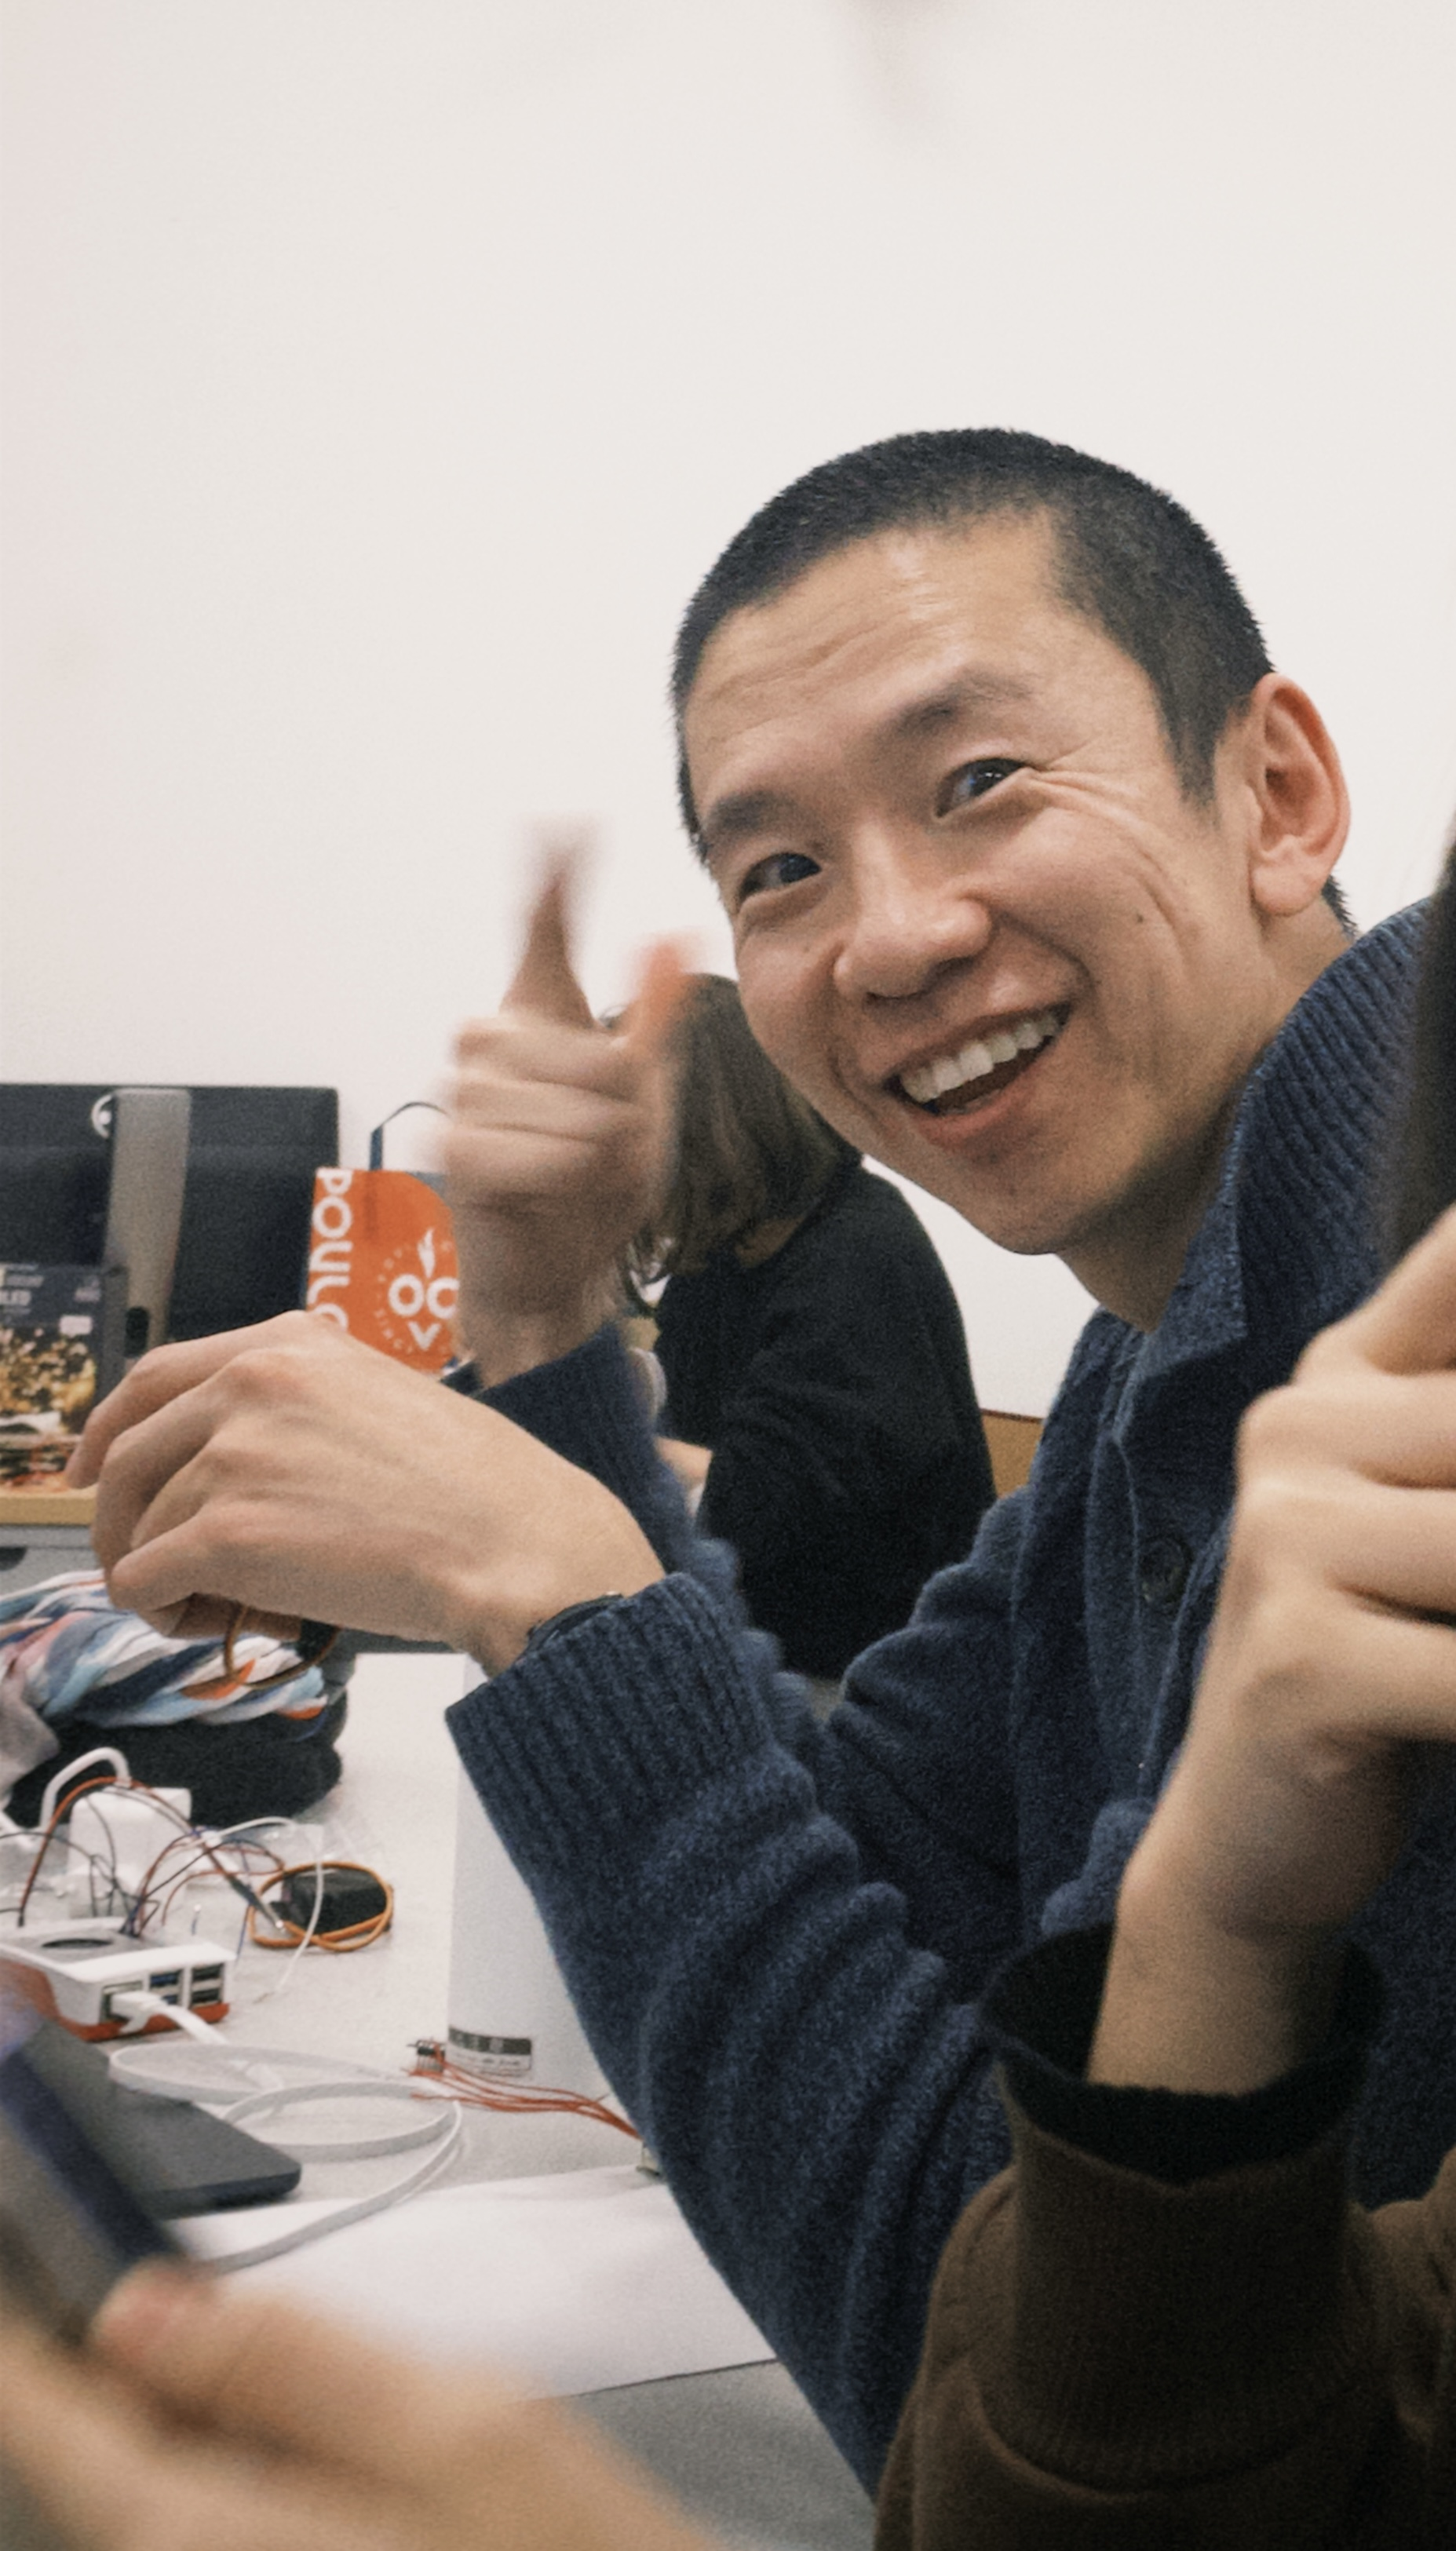
\includegraphics[width=2.37cm]{images/zhaoyu.jpg} &
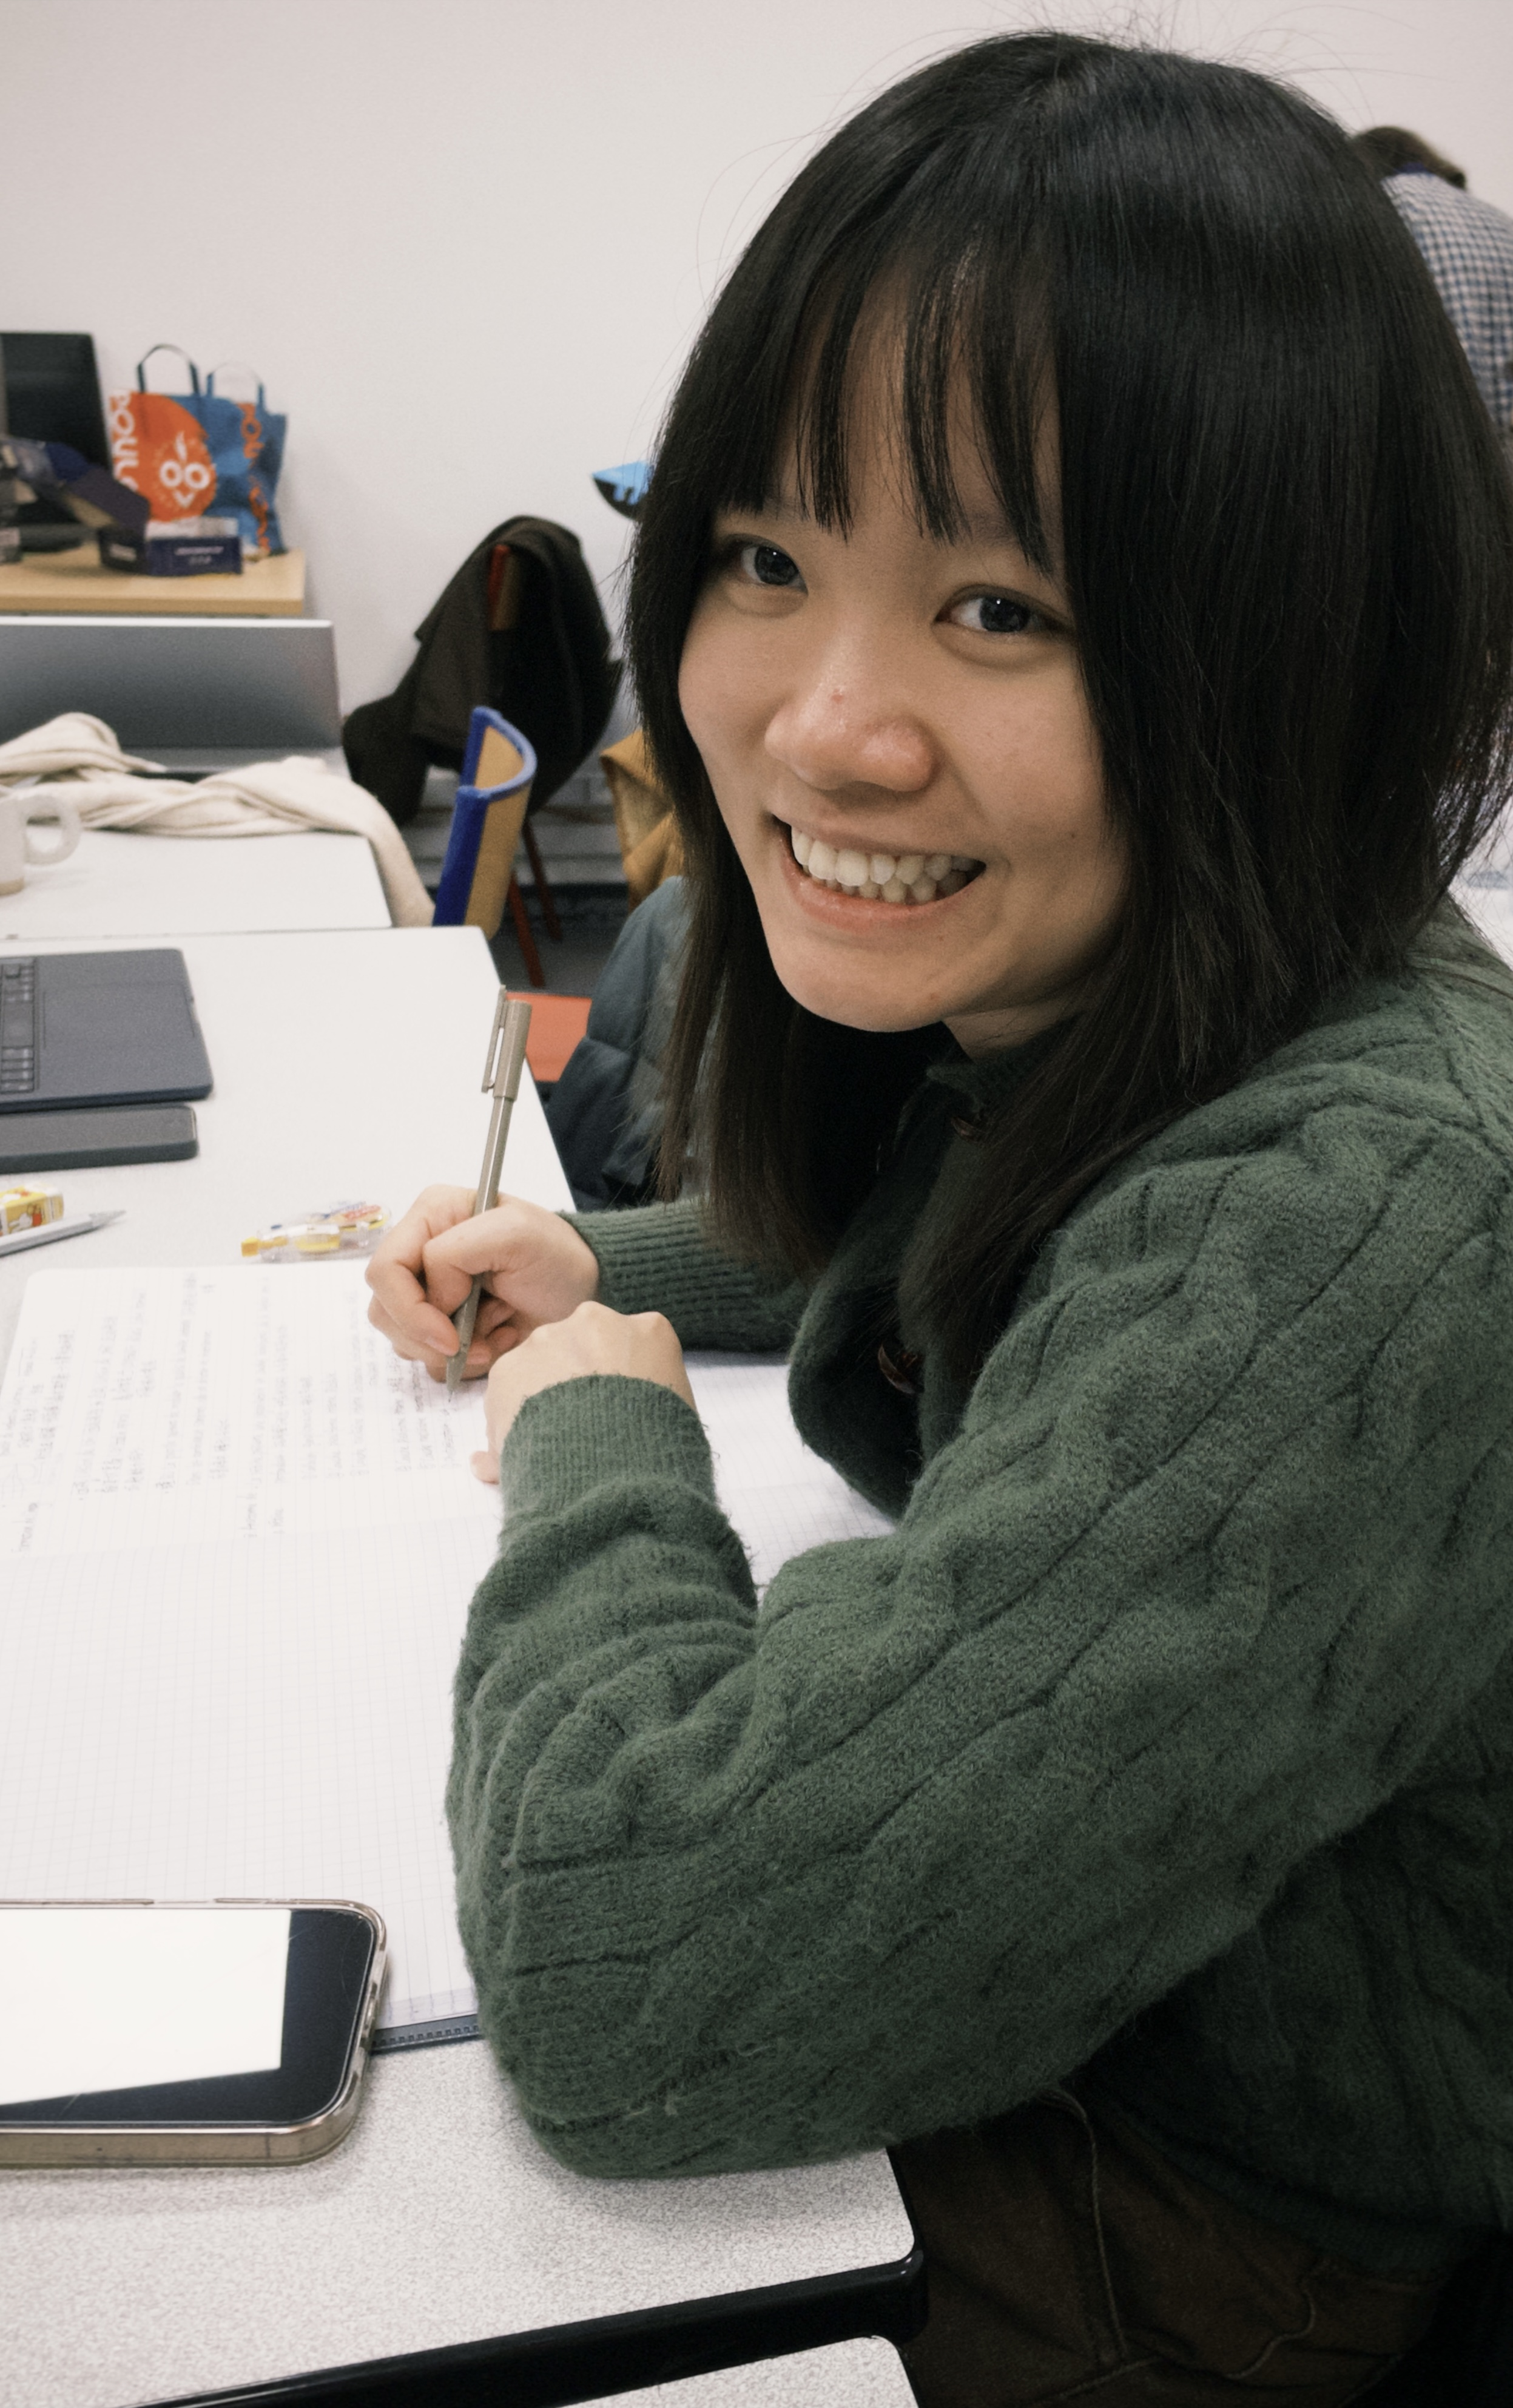
\includegraphics[width=2.62cm]{images/xinqi.jpg} &
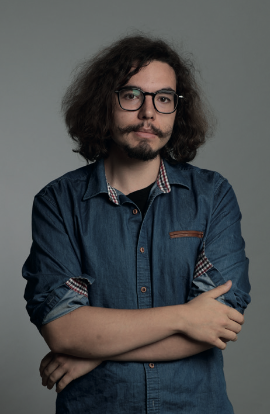
\includegraphics[width=2.68cm]{images/Lou.png} \\[0.2cm]

% Noms
\textbf{Lena BESSA} &
\textbf{Zhaoyu WANG} &
\textbf{Xinqi TANG} &
\textbf{Lou LOPEZ} \\

% Rôles (2 lignes max)
\begin{tabular}{c}
\scriptsize Chef de projet\\
Coordonne tout
\end{tabular}
&
\begin{tabular}{c}
\scriptsize Programmation\\
Câblage
\end{tabular}
&
\begin{tabular}{c}
\scriptsize Application Android\\
Interface user
\end{tabular}
&
\begin{tabular}{c}
\scriptsize Conception châssis\\
recherche
\end{tabular}
\\

\end{tabular}

\end{center}

\vspace{0.4cm}

\centering
\scriptsize
\textit{Tous les membres participent au montage et à l’intégration du prototype.}

\end{frame}



% -------------------------------------------------------------
% SLIDE: Problématique
\section{Problématique}

\begin{frame}{\textbf{Problématique}}

\begin{itemize}
    \item<1-> Fatigue physique importante liée au transport d’objets.
    \item<2-> Difficultés pour les personnes à mobilité réduite.
    \item<3-> Risques liés aux déplacements en intérieur.
    \item<4-> Manque de solutions compactes et stables.
\end{itemize}

\begin{alertblock}{Problème central}
Comment faciliter le transport d’objets en intérieur  
tout en garantissant stabilité et sécurité?
\end{alertblock}

\end{frame}

% -------------------------------------------------------------
% SLIDE: Présentation générale du projet
% -------------------------------------------------------------
\section{Objectifs}

\begin{frame}{\textbf{Objectifs du projet}}

\begin{block}{Objectif principal}
Concevoir un robot capable de transporter des objets légers
en environnement intérieur de manière stable et sécurisée.
\end{block}

\begin{itemize}
    \item<1-> Franchissement de petites marches.
    \item<2-> Pilotage via application mobile.
    \item<3-> Stabilisation de la charge.
    \item<4-> Sécurisation des déplacements.
\end{itemize}

\end{frame}


% -------------------------------------------------------------
% SLIDE : État de l’art
% -------------------------------------------------------------
\section{État de l’art}
% Slide 1
\begin{frame}{Plan de la présentation}
\tableofcontents[currentsection, ]
\end{frame}

% -------------------------------------------------------------
\begin{frame}{\textbf{Contexte sanitaire et robotique}}

\begin{itemize}
    \item Vieillissement rapide de la population mondiale.
    \item Manque croissant de personnel hospitalier.
    \item Développement du secteur robotique comme réponse structurelle
    \cite{bloss2011}.
\end{itemize}

\vspace{0.3cm}

\begin{block}{Impact COVID-19}
Transition accélérée vers la téléprésence et la robotisation des services
\cite{bourdon2023}.
\end{block}

\end{frame}

% -------------------------------------------------------------
% Slide 2
% -------------------------------------------------------------
\begin{frame}{Les robots d’assistance et leurs effets}

\begin{itemize}
    \item \textbf{Teng et al. (2022)} :
    revue systématique de 33 études —
    téléprésence, aide au diagnostic, distribution médicamenteuse.
    
    \item \textbf{Wang et al. (2024)} :
    revue de 31 robots médicaux,
    dont 9 dispositifs dédiés au transport.
    
    \item \textbf{Li et al. (2023)} :
    usage quotidien favorisant le mieux-être psychologique.
\end{itemize}

\end{frame}

% -------------------------------------------------------------
% Slide 3
% -------------------------------------------------------------
\begin{frame}{Robot TUG d’Aethon}

\begin{columns}

\column{0.55\textwidth}
\centering
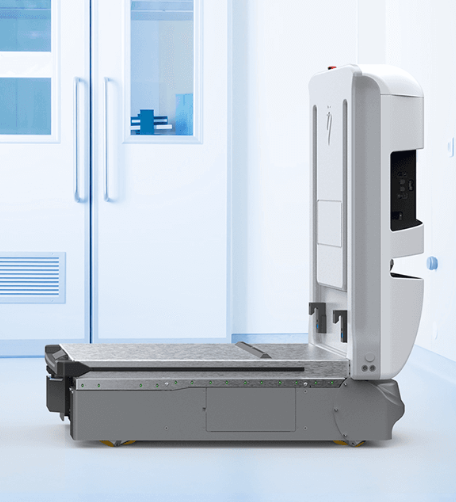
\includegraphics[width=5.5cm]{../img/tug.png}\\
{\scriptsize Source : aethon.com}

\column{0.45\textwidth}

\textbf{Avantages}
\begin{itemize}
    \item Transport autonome.
    \item Capacité jusqu’à 400 kg.
\end{itemize}

\vspace{0.2cm}

\textbf{Limites}
\begin{itemize}
    \item Robot très lourd.
    \item Incapable de monter des escaliers.
\end{itemize}

\end{columns}

\end{frame}

% -------------------------------------------------------------
% Slide 4
% -------------------------------------------------------------
\begin{frame}{Robot Care-O-Bot}

\begin{columns}

\column{0.55\textwidth}
\centering
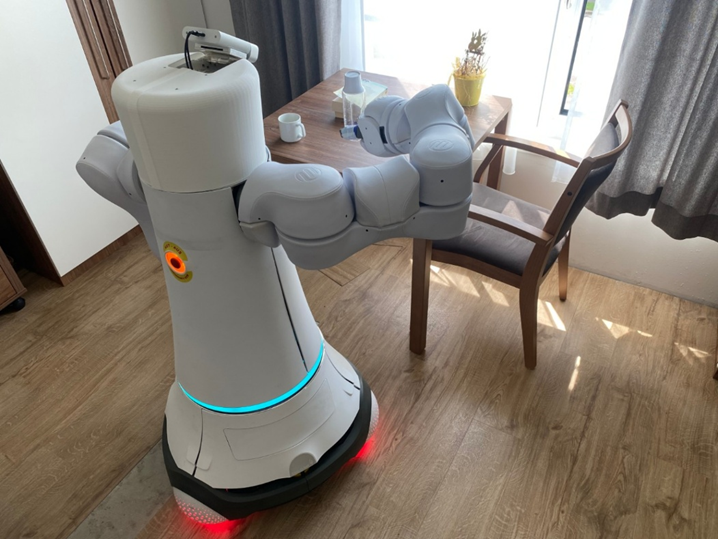
\includegraphics[width=5cm]{../img/care-o-bot.png}\\
{\scriptsize Source : care-o-bot.de}

\column{0.45\textwidth}

\textbf{Avantages}
\begin{itemize}
    \item Apparence sociale et sympathique.
    \item Bras mécanisés.
    \item Polyvalence fonctionnelle.
\end{itemize}

\vspace{0.2cm}

\textbf{Limites}
\begin{itemize}
    \item Capacité limitée ($\approx$5 kg).
    \item Complexité et coût élevés.
\end{itemize}

\end{columns}

\end{frame}

% -------------------------------------------------------------
% Slide 5
% -------------------------------------------------------------
\begin{frame}{Labrador Retriever Robot}

\begin{columns}

\column{0.55\textwidth}
\centering
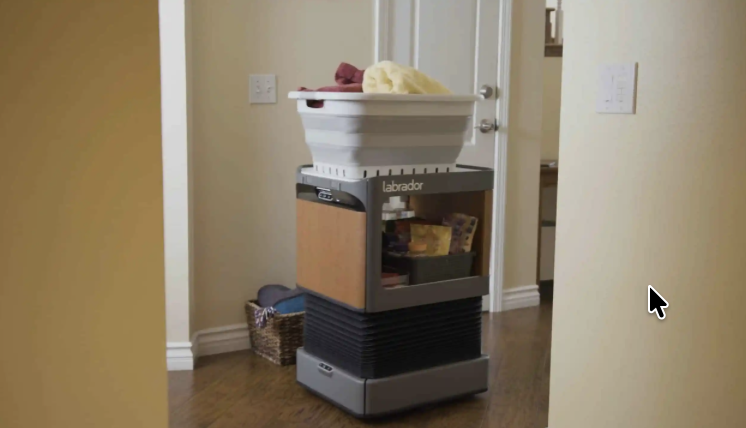
\includegraphics[width=5cm]{../img/labrador.png}\\
{\scriptsize Source : labradorsystems.com}

\column{0.45\textwidth}

\textbf{Avantages}
\begin{itemize}
    \item Polyvalent.
    \item Transport jusqu’à 11 kg.
    \item Manipulation plateau repas.
\end{itemize}

\vspace{0.2cm}

\textbf{Limites}
\begin{itemize}
    \item Coût élevé ($\approx$6900 \$).
    \item Ne monte pas les escaliers.
\end{itemize}

\end{columns}

\end{frame}

% -------------------------------------------------------------
% Slide 6
% -------------------------------------------------------------
\begin{frame}{2. Les défis identifiés}

Après analyse des robots existants, CarryBot doit :

\begin{itemize}
    \item Être capable de \textbf{monter les escaliers}.
    \item Être capable de \textbf{s’auto-rééquilibrer rapidement}.
\end{itemize}

\begin{alertblock}{Objectif stratégique}
Combiner mobilité verticale + stabilité active
dans un format compact.
\end{alertblock}

\end{frame}

% -------------------------------------------------------------
% Slide 7
% -------------------------------------------------------------
\begin{frame}{Monter les escaliers}

\begin{itemize}
    \item \textbf{Seo et al. (2023)} :
    défi majeur en robotique de service intérieur.
    \item DARPA Robotics Challenge (2015) :
    taux de réussite $\approx$ 30\%.
    \item Forte variabilité géométrique des escaliers
    (hauteur, angle, contexte culturel).
\end{itemize}

\vspace{0.3cm}

\textbf{Catégories identifiées :}
\begin{itemize}
    \item Robots à chenilles.
    \item Robots à pattes.
    \item Robots à roues et liaisons.
    \item Robots hybrides roues-pattes.
\end{itemize}

\end{frame}

% -------------------------------------------------------------
% Slide 8
% -------------------------------------------------------------
\begin{frame}{Robot ROSA}

\begin{columns}

\column{0.55\textwidth}
\centering
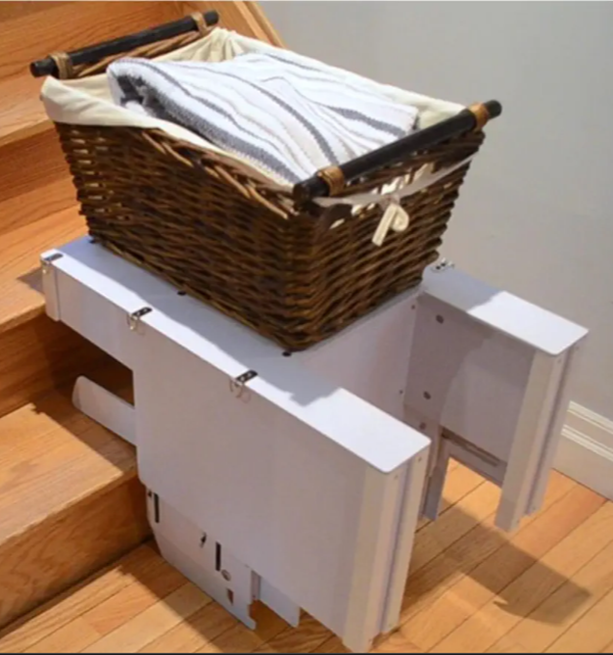
\includegraphics[width=5cm]{../img/rosa.png}\\
{\scriptsize Source : robotshop.com}

\column{0.45\textwidth}

\textbf{Avantages}
\begin{itemize}
    \item Léger (20 kg).
    \item Charge jusqu’à 25 kg.
    \item Conception simple.
\end{itemize}

\vspace{0.2cm}

\textbf{Limites}
\begin{itemize}
    \item Mouvements saccadés.
    \item Prix élevé ($\approx$3900 \$).
    \item Usage restreint aux escaliers.
\end{itemize}

\end{columns}

\end{frame}

% -------------------------------------------------------------
% Slide 9
% -------------------------------------------------------------
\begin{frame}{S’auto-équilibrer}

\begin{itemize}
    \item \textbf{Salwa \& Krzysztofik (2025)} :
    modèle du \textbf{pendule inversé}.
    
    \item Système intrinsèquement instable.
    
    \item Système \textbf{sous-actionné} :
    moins d’actionneurs que de degrés de liberté.
    
    \item Forte exigence de précision temporelle.
\end{itemize}

\end{frame}

% -------------------------------------------------------------
% Slide 10
% -------------------------------------------------------------
\begin{frame}{Wheelchair.q}

\begin{columns}

\column{0.45\textwidth}
\centering
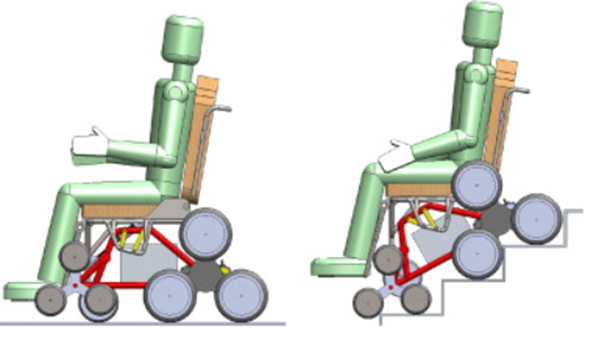
\includegraphics[width=5cm]{../img/wheel.png}\\
{\scriptsize Source: Quaglia et al., 2011}

\column{0.55\textwidth}

\textbf{Avantages}
\begin{itemize}
    \item Rééquilibrage mécanique.
    \item Solution légère et efficace.
\end{itemize}

\vspace{0.2cm}

\textbf{Limites}
\begin{itemize}
    \item Stratégie d’équilibre identique
    quel que soit le poids utilisateur.
\end{itemize}

\end{columns}

\end{frame}


%-- Positionnement différenciant de CarryBot
\begin{frame}{\textbf{Positionnement différenciant de CarryBot}}
\begin{itemize}
    \item<1-> Conception centrée sur les besoins domestiques.
    \item<2-> Mécanisme de roues Tri-Star pour franchissement de marches.
    \item<3-> Stabilisation active via vérin linéaire.
    \item<4-> Interface de pilotage simple et intuitive.
    \item<5-> Sécurisation renforcée (arrêt d’urgence physique et logiciel).
\end{itemize}
\end{frame} 

% -------------------------------------------------------------
% SLIDE Analyse des besoins
% -------------------------------------------------------------
\section{Analyse des besoins}
\begin{frame}{\textbf{Analyse des besoins}}

\begin{itemize}
    \item Déplacement fluide en couloirs et pièces étroites.
    \item Stabilité lors des changements de niveau.
    \item Interface simple et accessible.
    \item Autonomie suffisante.

    \item Deux modes de pilotage attendus:
    \begin{itemize}
        \item \textbf{Pilotage manuel} via l’application Android (pictogrammes simples).
        \item \textbf{Pilotage automatique} via \textbf{suivi de lignes au sol}.
    \end{itemize}
    \item Besoin de \textbf{sécurisation forte}: arrêt d’urgence physique
    + arrêt logiciel sur l’application.
\end{itemize}

\end{frame}

% -------------------------------------------------------------
% SLIDE : Limitation temporelle
% -------------------------------------------------------------
\begin{frame}{\textbf{Limites du périmètre actuel}}

\begin{block}{Fonctionnalité initialement prévue}
Le mode de pilotage automatique par \textbf{suivi de ligne au sol}
était intégré dans le cahier des charges initial.
\end{block}

\vspace{0.3cm}

\begin{alertblock}{Arbitrage projet}
En raison des contraintes temporelles liées :
\begin{itemize}
    \item à l’assemblage mécanique,
    \item à l’intégration électronique,
    \item aux tests de stabilisation et de sécurité,
\end{itemize}

la fonctionnalité de suivi de ligne n’a pas pu être implémentée
dans la version actuelle du prototype.
\end{alertblock}

\end{frame}

% -------------------------------------------------------------
% SLIDE : Personas
% -------------------------------------------------------------
\begin{frame}{\textbf{Persona 1 — Marie, 73 ans}}

\begin{columns}

\column{0.55\textwidth}
\centering
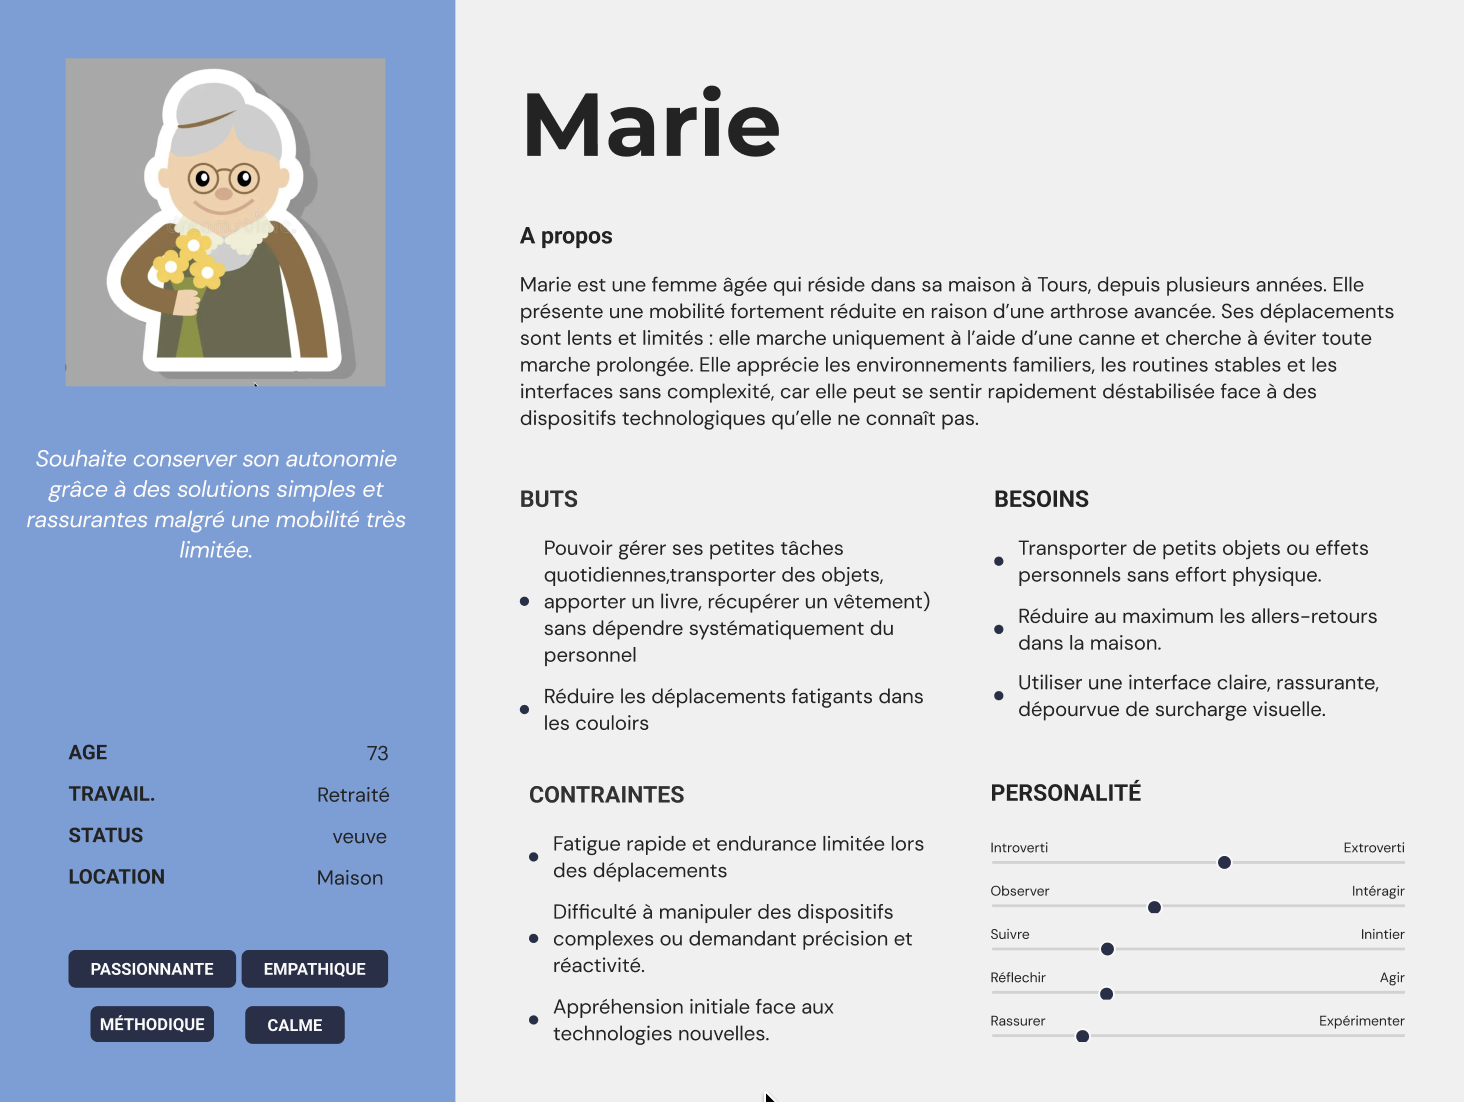
\includegraphics[width=6.2cm]{../img/marie.png}

\column{0.45\textwidth}

\textbf{Profil}
\begin{itemize}
    \item retraitée vit dans sa maison
    \item Mobilité réduite due à une arthrose sévère
    \item Fatigue rapide lors des déplacements
\end{itemize}

\vspace{0.1cm}

\textbf{Scénario d’usage}
\begin{block}{« Déposer un objet puis guider CarryBot »}
Marie pose une bouteille ou un petit objet sur CarryBot.  
Elle utilise l’application Android pour piloter le robot jusqu’au couloir.  
\end{block}

\end{columns}
\end{frame}



% -------------------------------------------------------------
\begin{frame}{\textbf{Persona 2 — Luca, 34 ans}}

\begin{columns}

\column{0.55\textwidth}
\centering
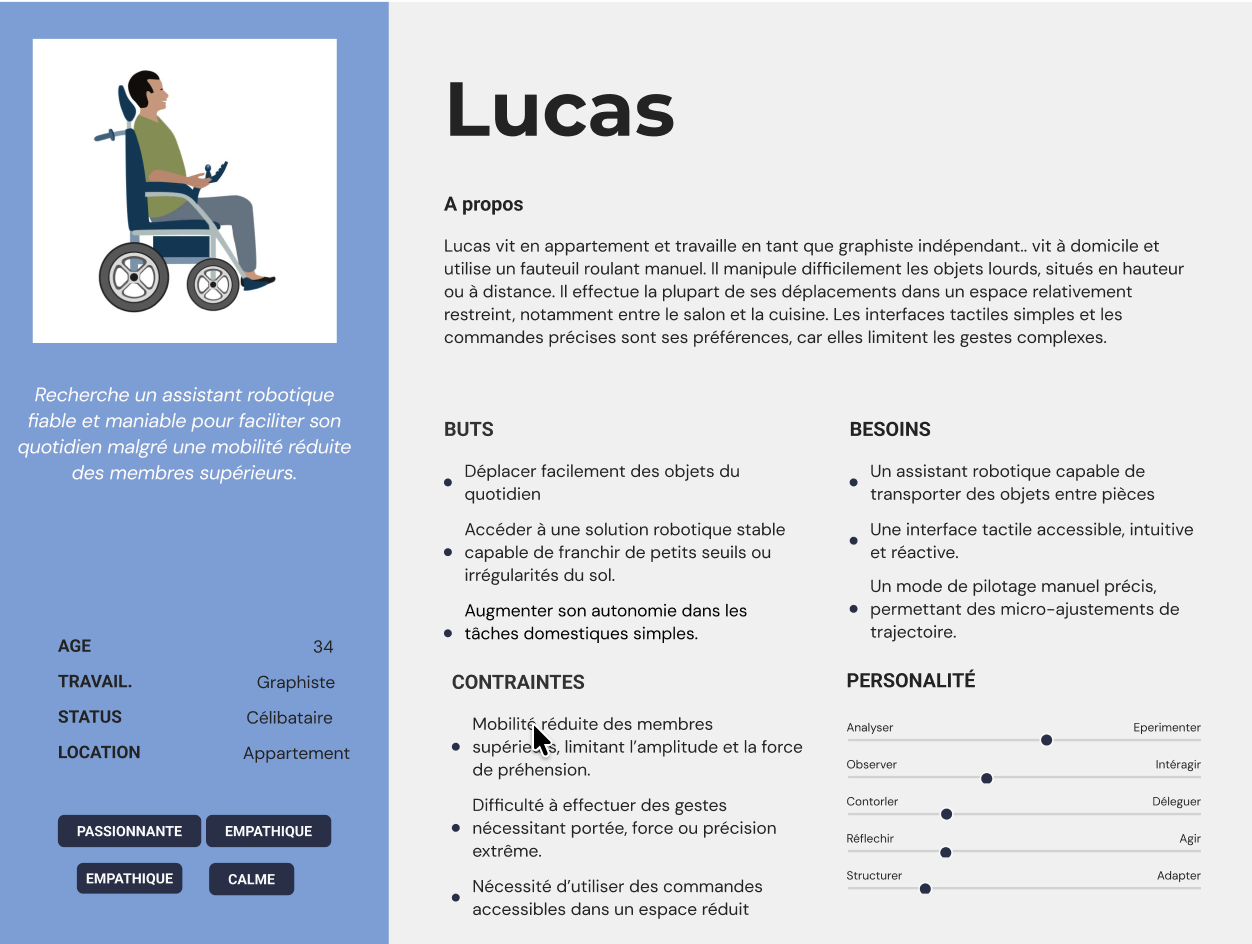
\includegraphics[width=6.2cm]{../img/lucas.png}

\column{0.45\textwidth}

\textbf{Profil}
\begin{itemize}
    \item En fauteuil manuel
    \item Difficulté à transporter un plateau tout en se déplaçant
\end{itemize}

\vspace{0.2cm}

\textbf{Scénario d’usage}
\begin{block}{« Transporter un plateau sans gêner la conduite du fauteuil »}
Luca dépose son plateau sur CarryBot.  
Il contrôle ensuite le robot via l’application Android pour l’amener  
du plan de travail au salon.  
\end{block}

\end{columns}
\end{frame}

% -------------------------------------------------------------
% SLIDE: Public cible
% -------------------------------------------------------------

\begin{frame}{\textbf{Public cible}}

\begin{itemize}
    \item<1-> Personnes âgées (fragilité motrice, risque de chute).
    \item<2-> Personnes à mobilité réduite (PMR).
    \item<3-> Patients en centres de rééducation.
    \item<4-> Infirmiers, aide-soignants, personnels hospitaliers.
    \item<5-> Structures médico-sociales: EHPAD, foyers de vie.
\end{itemize}

\end{frame}

% -------------------------------------------------------------
% SLIDE Architecture CarryBot (images à mettre)
% -------------------------------------------------------------
\section{Architecture du CarryBot}
\begin{frame}{\textbf{Architecture du CarryBot}}

\begin{columns}
\column{0.5\textwidth}
\centering
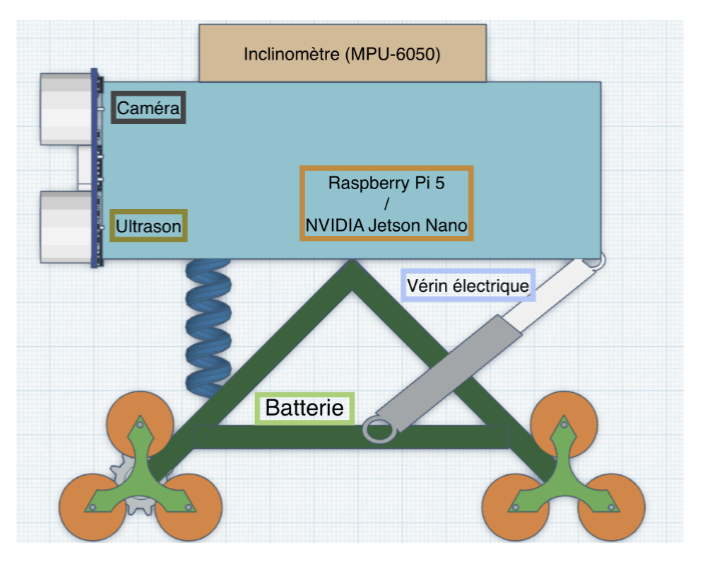
\includegraphics[width=5cm]{../img/CB-global.png}\\
\footnotesize Vue globale du robot

\column{0.5\textwidth}
\centering
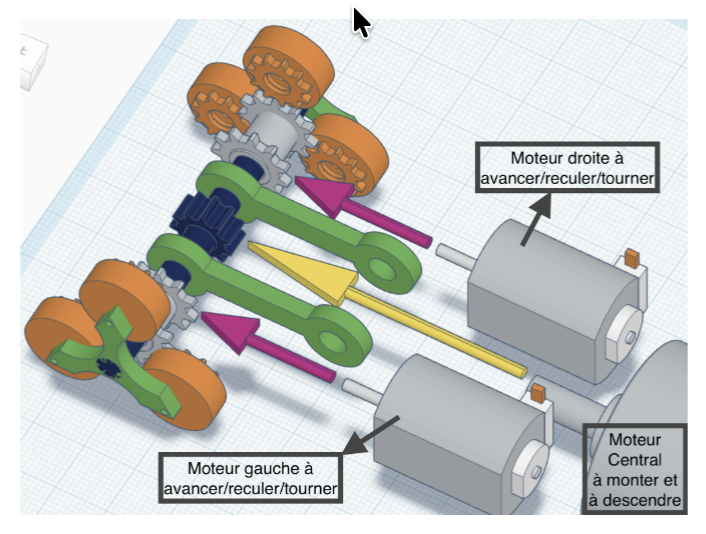
\includegraphics[width=5cm]{../img/CB-detail.png}\\
\footnotesize Mécanisme Tri-Star
\end{columns}

\end{frame}


% -------------------------------------------------------------
% SLIDE Matériel
% -------------------------------------------------------------
\section{Composants matériels}
\begin{frame}{\textbf{Composants matériels}}

\begin{columns}

% ------- Colonne gauche: texte -------
\column{0.65\textwidth}
\begin{itemize}
    \item Raspberry Pi 5 + caméra Intel RealSense.
    \item 1 Carte Makeblock MegaPi.
    \item 1 Capteurs ultrason + IMU.
    \item 4 Roues Tri-Star imprimées en 3D.
    \item 1 Vérin linéaire pour stabilisation (12V).
    \item 2 Boutons STOP physiques.
    \item 4 Moteur DC 9V.
\end{itemize}

% ------- Colonne droite: image -------
\column{0.35\textwidth}
\centering
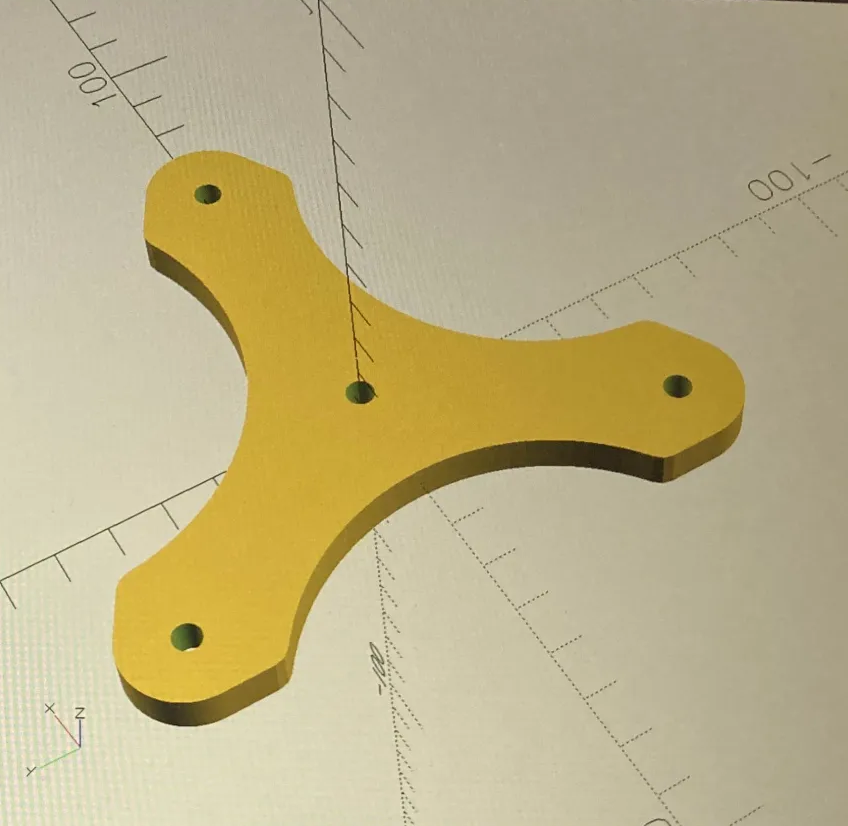
\includegraphics[width=0.9\linewidth]{images/tri-star.png}\\
{\scriptsize\textit{tri-star du robot en 3D}}
\end{columns}

\end{frame}

%-------------------------------------------------------------

\begin{frame}{\textbf{Architecture globale}}

\begin{columns}

\column{0.5\textwidth}
\centering
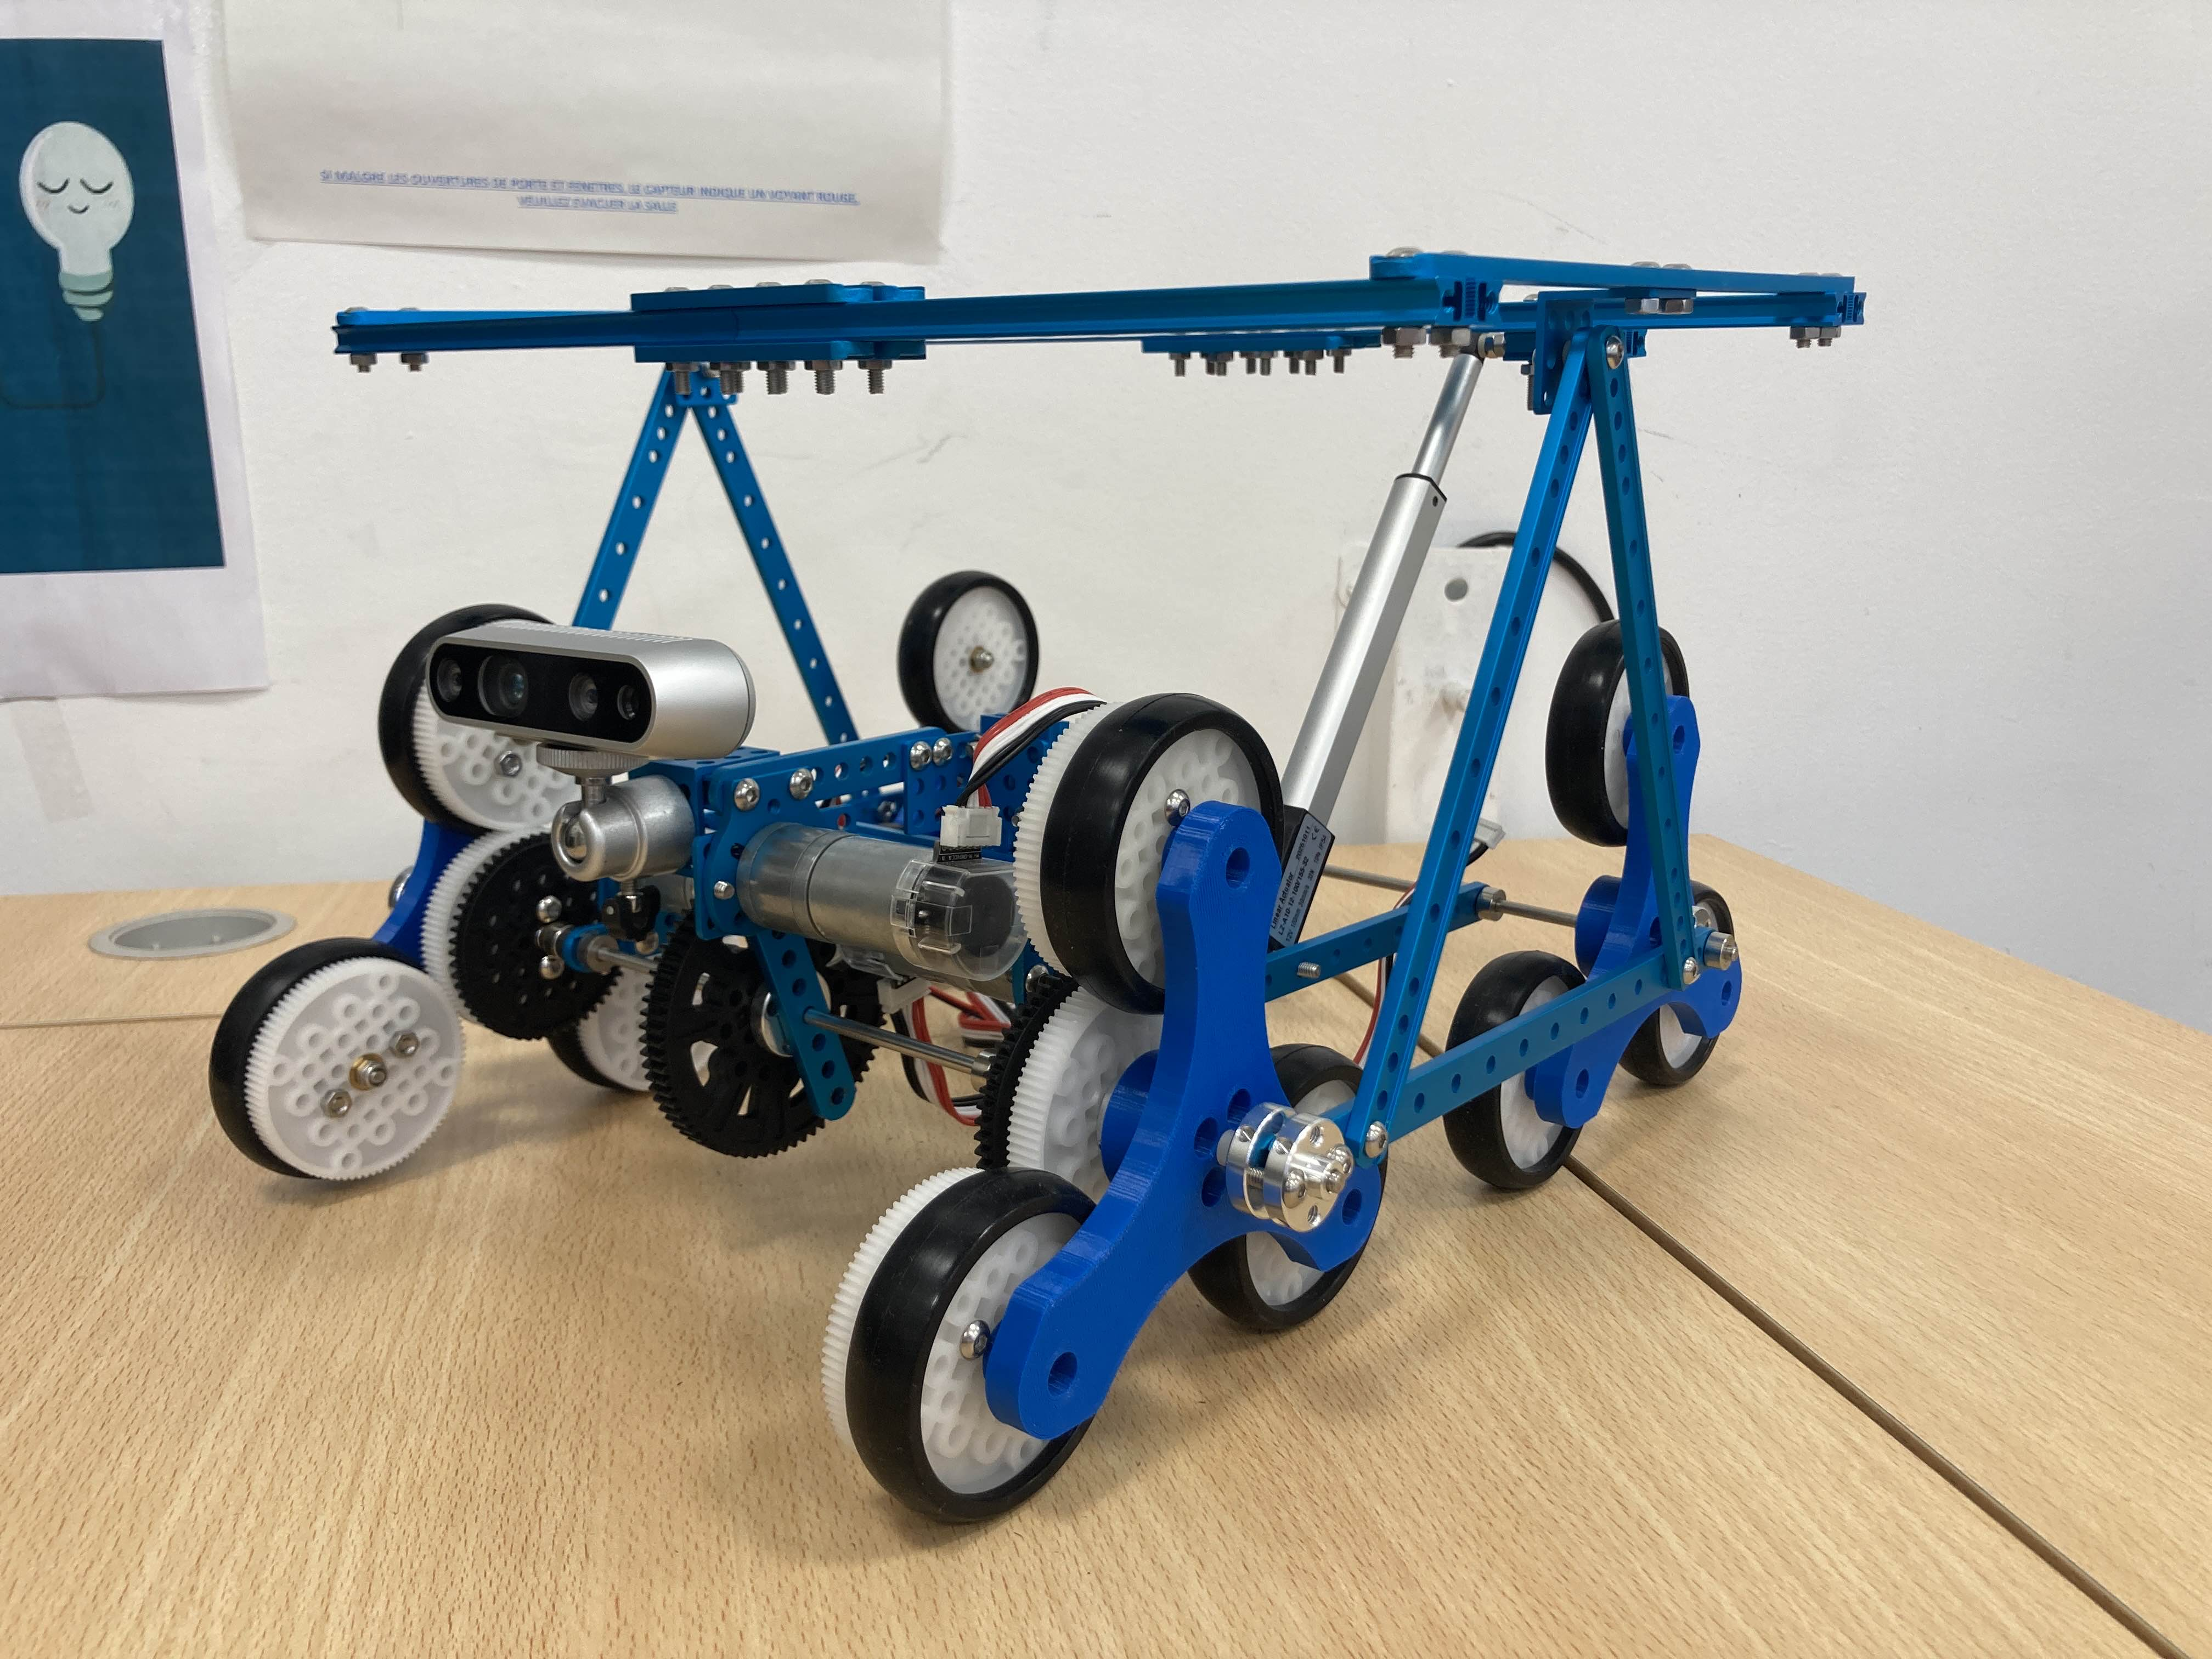
\includegraphics[width=5cm]{images/carryBot.jpg}\\
{\scriptsize Prototype actuel}

\column{0.5\textwidth}

\begin{itemize}
    \item Châssis modulaire.
    \item Roues Tri-Star.
    \item Vérin de stabilisation.
    \item Capteurs et caméra.
\end{itemize}

\end{columns}

\end{frame}

% -------------------------------------------------------------
% SLIDE Logique
% -------------------------------------------------------------

\section{Logique de contrôle}

\begin{frame}{\textbf{Du capteur à l’actionneur : Raspberry Pi}}

\begin{block}{Rôle principal}
Agir comme \textbf{cerveau décisionnel} du système.
\end{block}

\begin{itemize}
    \item Traite les données caméra (vision + profondeur).
    \item Prend les décisions de déplacement (détection de murs/escaliers).
    \item Expose les services \textbf{HTTP} (interface \textbf{Web/API}) pour le pilotage à distance.
    \item Diffuse un \textbf{flux vidéo} en temps réel pour la supervision.
    \item Communique avec MegaPi (envoi des commandes, réception de la télémétrie).
    \item Assure la connectivité réseau en \textbf{Wi-Fi} (mode point d’accès).
\end{itemize}

\begin{alertblock}{Entrées / sorties}
Entrées : caméra + télémétrie MegaPi \hspace{0.3cm} Sorties : commandes moteurs.
\end{alertblock}

\end{frame}


\begin{frame}{\textbf{Du capteur à l’actionneur : MegaPi}}

\begin{block}{Rôle principal}
Exécuter les commandes bas niveau et piloter les actionneurs.
\end{block}

\begin{itemize}
    \item Contrôle les moteurs de roues et du mécanisme Tri-Star.
    \item Lecture des capteurs embarqués (ultrason, IMU).
    \item Renvoie au Raspberry Pi les données de télémétrie.
    \item Gestion de l’exécution temps réel des ordres reçus.
    \item Ajuste l’équilibre en pilotant le vérin à partir des données IMU.
\end{itemize}

\begin{alertblock}{Résultat}
Transformation de la décision logicielle en mouvement physique du robot.
\end{alertblock}

\end{frame}



% -------------------------------------------------------------
% SLIDE Application Android
% -------------------------------------------------------------
\section{Application}

\begin{frame}{\textbf{Application Android}}

\begin{columns}

\column{0.5\textwidth}
\centering
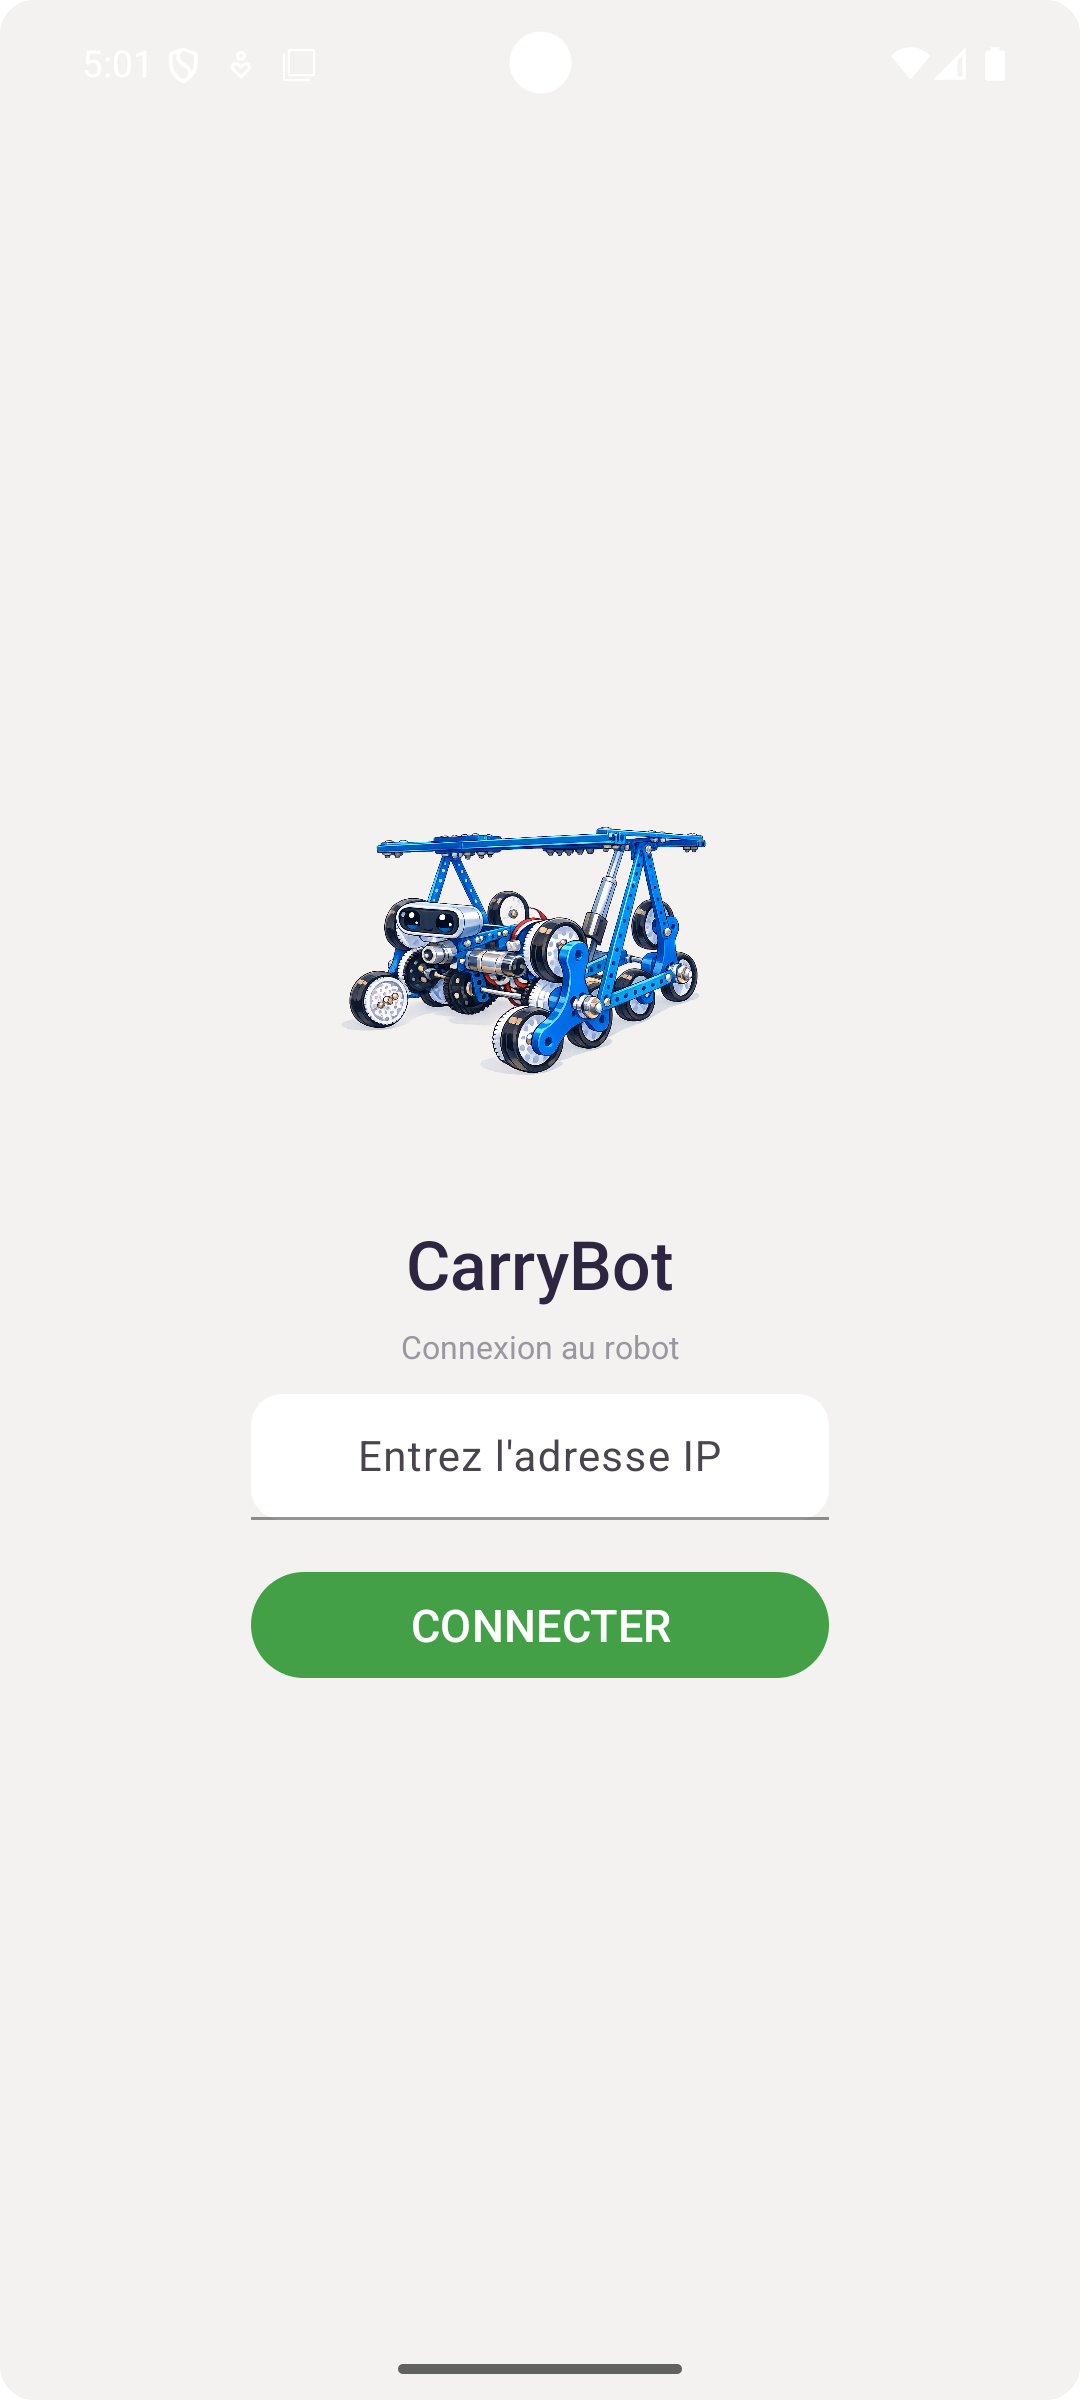
\includegraphics[width=2.6cm]{images/accueil.png}\\
{\scriptsize Connexion}

\column{0.5\textwidth}
\centering
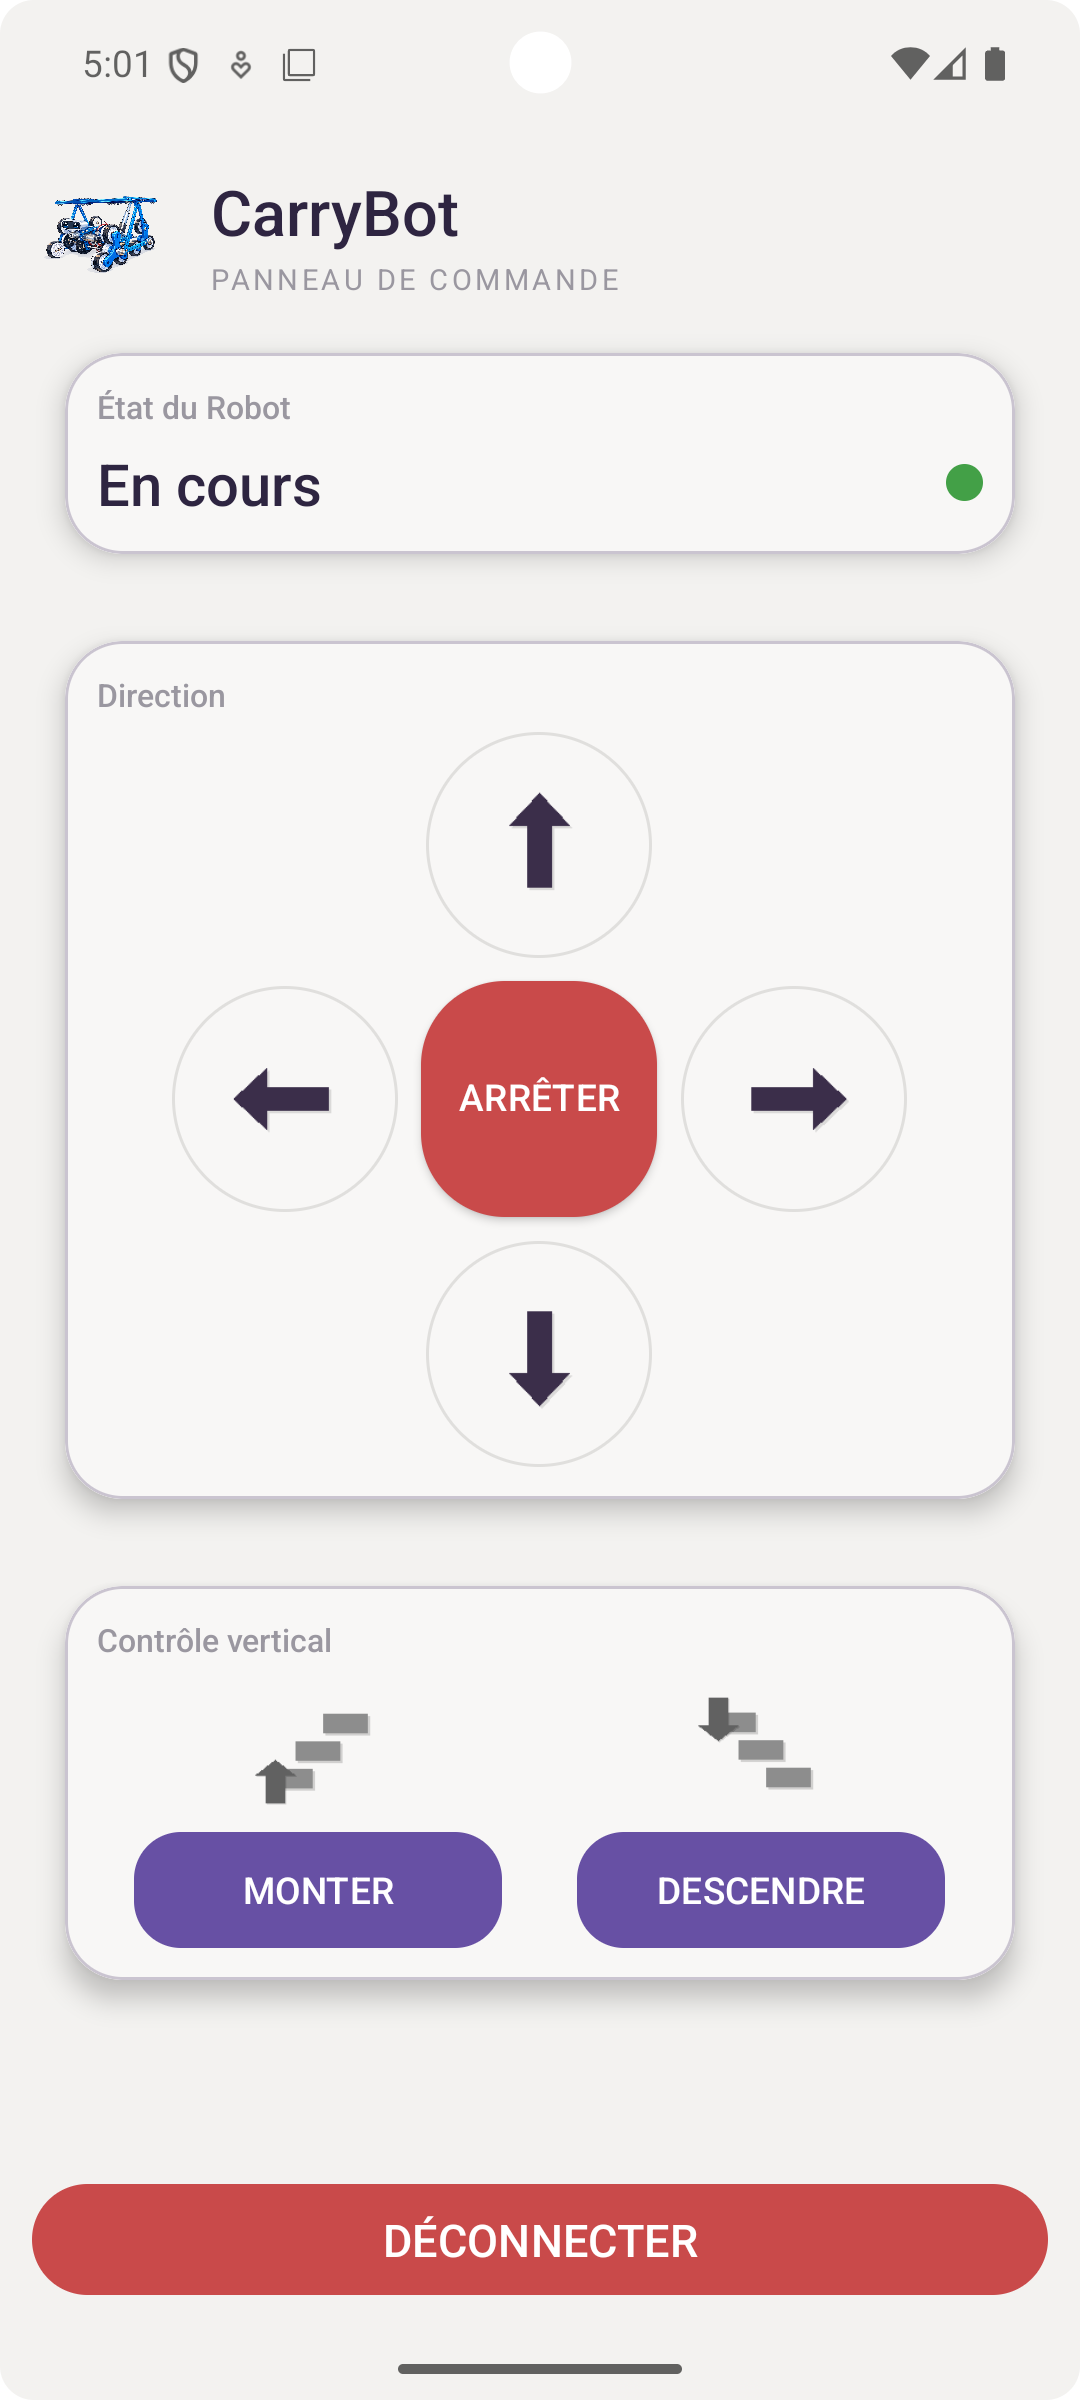
\includegraphics[width=2.6cm]{images/interface-Collab.png}\\
{\scriptsize Pilotage}

\end{columns}

\vspace{0.3cm}

\begin{itemize}
    \item Connexion par IP.
    \item Commandes directionnelles.
    \item Mode monter/descendre de marches.
    \item Bouton d’arrêt logiciel.
\end{itemize}

\end{frame}


% =============================================================
% SLIDE: Technologies utilisées
% =============================================================

\section{Technologies}

\begin{frame}{\textbf{Technologies utilisées}}

\begin{block}{Traitement caméra}

\begin{itemize}
    \item \textbf{pyrealsense2}: accès aux données de profondeur.
    \item \textbf{OpenCV2}: traitement d’image et détection.
    \item \textbf{NumPy}: calculs matriciels et analyse des données.
\end{itemize}

\end{block}

\begin{block}{Commande des moteurs}

\begin{itemize}
    \item \textbf{pyserial}: communication série avec la carte.
    \item \textbf{threading}: gestion multitâche.
    \item \textbf{MeMegaPi.h}: pilotage moteurs (Makeblock MegaPi).
\end{itemize}

\end{block}

\begin{block}{Surveillance et contrôle web}

\begin{itemize}
    \item \textbf{http.server}: serveur web embarqué.
    \item \textbf{socketserver}: gestion des connexions réseau.
\end{itemize}

\end{block}

\end{frame}


% -------------------------------------------------------------
% SLIDE Exigences
% -------------------------------------------------------------
\section{Exigences principales}
\begin{frame}{\textbf{Exigences principales}}

\begin{block}{Fonctionnelles}
\begin{itemize}
    \item  Pilotage manuel.
    \item  Arrêt d’urgence.
    \item  Franchissement petites marches.
\end{itemize}
\end{block}

\begin{block}{Qualité}
\begin{itemize}
    \item Sécurité.
    \item Stabilité.
    \item Autonomie 1h (the current Prototype).
\end{itemize}
\end{block}

\end{frame}




\section{Avancement}

\begin{frame}{\textbf{État d’avancement}}

\begin{block}{Réalisations}

\begin{itemize}

\item \textbf{Mécanique}
\begin{itemize}
    \item Assemblage en cours.
    \item Ajustement du châssis.
    \item Stabilisation de la structure.
\end{itemize}

\item \textbf{Électronique}
\begin{itemize}
    \item Intégration capteurs.
    \item Installation moteurs et vérin.
    \item Câblage principal.
\end{itemize}

\item \textbf{Logiciel embarqué}
\begin{itemize}
    \item Gestion moteurs.
    \item Pilotage du vérin.
    \item Détection murs et escaliers (caméra).
\end{itemize}

\item \textbf{Application}
\begin{itemize}
    \item Refonte interface.
    \item Ajout visuels.
    \item Amélioration ergonomie.
\end{itemize}

\end{itemize}

\end{block}

\end{frame}

% =============================================================

% =============================================================
\section{Détection par caméra}

\begin{frame}{\textbf{Détection des murs}}

\begin{columns}

\column{0.6\textwidth}
\centering
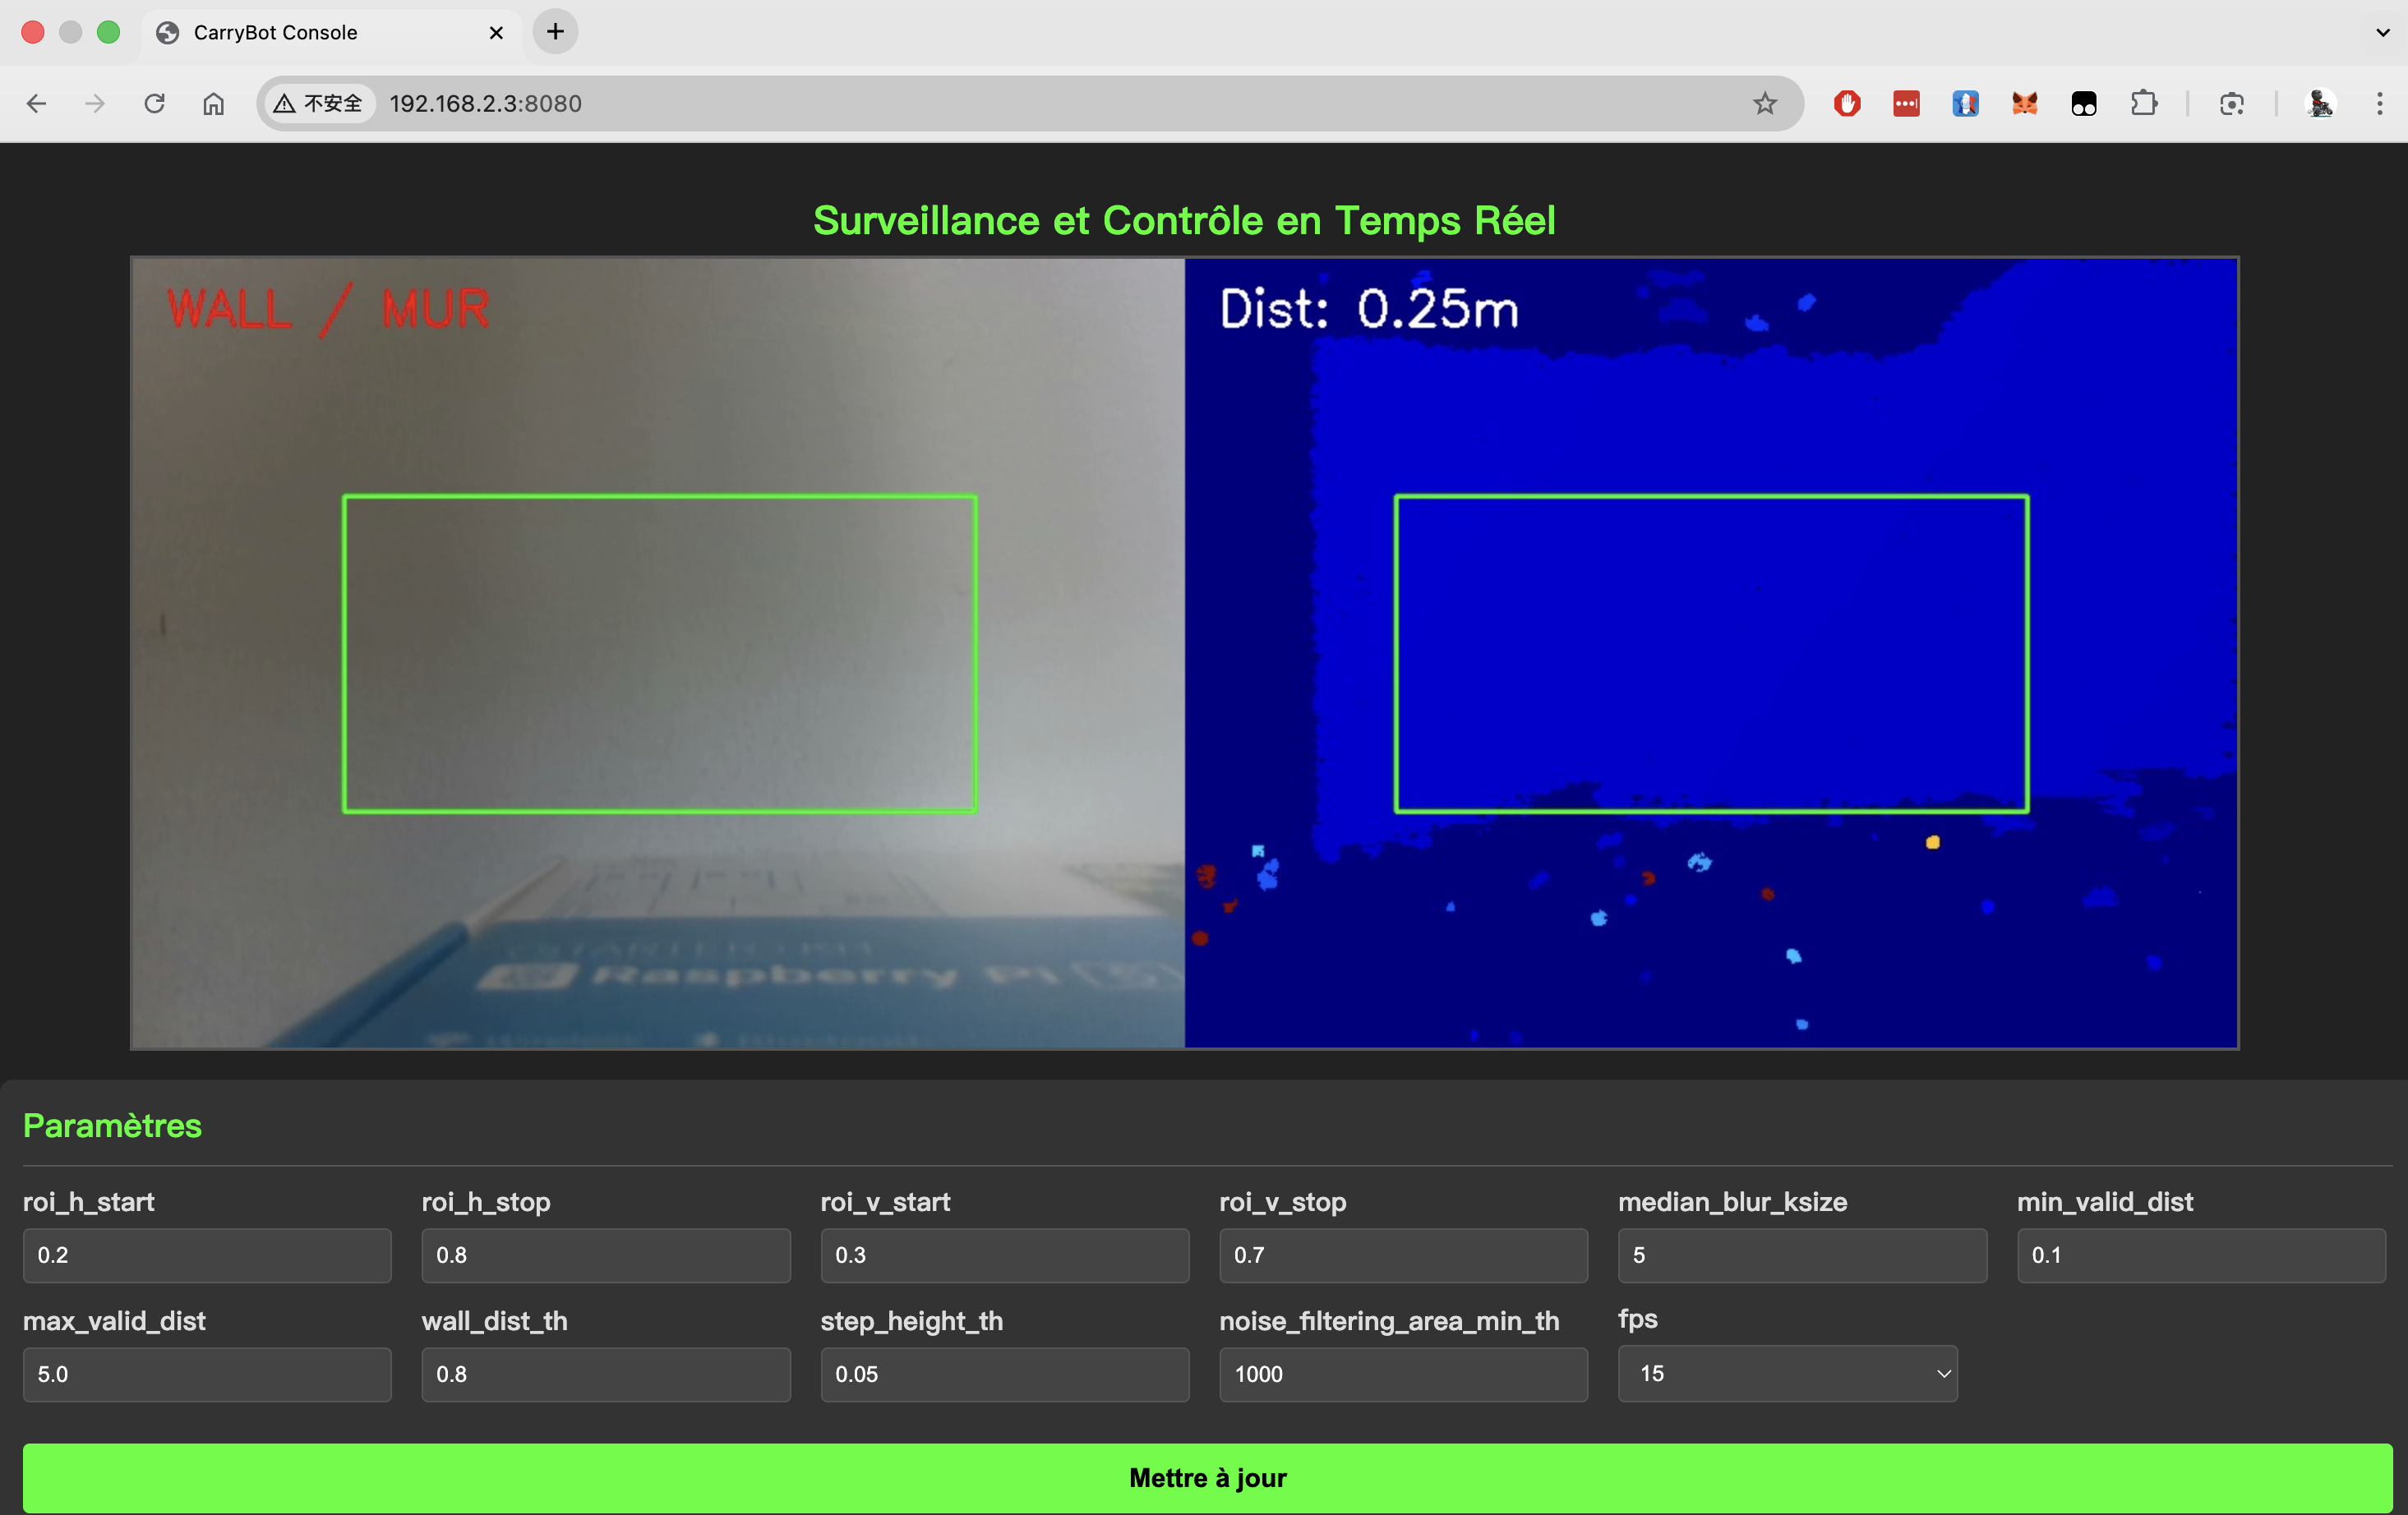
\includegraphics[width=\linewidth]{images/camera.png}\\
{\scriptsize Interface de détection mur via caméra RealSense}

\column{0.4\textwidth}

\begin{itemize}
    \item Utilisation de la caméra Intel RealSense.
    \item Analyse de la profondeur.
    \item Définition d’une zone d’intérêt (ROI).
    \item Calcul de distance moyenne.
    \item Classification mur / obstacle / escalier.
\end{itemize}

\end{columns}

\vspace{0.2cm}

\begin{block}{Fonctionnement}
Le système analyse la profondeur dans une zone centrale afin de détecter
la présence d’un mur et d’adapter le comportement du robot.
\end{block}

\end{frame}
% -------------------------------------------------------------
% SLIDE Perspectives
% -------------------------------------------------------------

\section{Perspectives}

\begin{frame}{\textbf{Perspectives}}

\begin{block}{Développements à venir}

\begin{itemize}
    \item Suivi de ligne.

\end{itemize}

\end{block}
\end{frame}


%--------------------------------------------------------------
\section{Bibliographie}
%--------------------------------------------------------------
\begin{frame}[allowframebreaks]{Bibliographie}
\footnotesize
\bibliography{references}
\end{frame}


% -------------------------------------------------------------
% SLIDE Finale
% -------------------------------------------------------------
\begin{frame}
\centering
\Huge \textbf{Merci pour votre attention}\\[0.5cm]
\Large Questions?
\end{frame}

\end{document}
